\documentclass[12pt,a4paper]{article}
\usepackage[utf8]{inputenc}
\usepackage[T1]{fontenc}
\usepackage{libertinus}
\usepackage[brazil]{babel}
\usepackage{indentfirst}       
\renewcommand{\familydefault}{\sfdefault}
\usepackage{amsmath, amssymb, amsthm, mathtools}
\usepackage{graphicx}
\usepackage{booktabs}
\usepackage{hyperref}
\usepackage[margin=2.5cm]{geometry}
\usepackage{titlesec}
\usepackage{microtype}
\usepackage{float}
\usepackage{xcolor}
\usepackage[colorlinks=true, urlcolor=blue, linkcolor=black, citecolor=black]{hyperref}
\linespread{1.15}
\setlength{\parskip}{10pt}
\setlength{\parindent}{0pt}
\titleformat{\section}{\Large\bfseries}{\thesection.}{0.6em}{}
\titleformat{\subsection}{\large\bfseries}{\thesubsection.}{0.6em}{}
\titlespacing*{\section}{0pt}{1.8em}{0.8em}
\titlespacing*{\subsection}{0pt}{1.4em}{0.6em}

\newtheorem{proposicao}{Proposição}
\newtheorem{lema}{Lema}
\renewcommand{\proofname}{Prova}

\begin{document}

\title{Modelo de organização educacional com grafos bipartidos}
\author{
  Carolina Chamon Torres Lima Abreu, Eduardo Antonio Pina Frias, \\
  Leonardo Henrique Melo Ruiz e Maximus Lemos Campero \\
  \small Fundação Getúlio Vargas -- EMAp \\
  \small Professora: Maria Soledad Aronna
}
\date{Rio de Janeiro -- RJ, 2026}

\maketitle

\section{Introdução}

O acesso à educação de qualidade no Brasil é um problema complexo que exige
soluções urgentes. Acreditamos que o modelo atual favorece a hiperconcentração
de professores altamente qualificados em um grupo restrito de instituições,
deixando muitas escolas sem acesso a profissionais de excelência. Esse cenário
priva estudantes com grande potencial de ter um impulso inicial necessário para
desenvolver suas carreiras.

Baseado nisso, propomos então o desenvolvimento de um modelo para maximizar a
qualidade geral dos profissionais nas instituições de ensino, o modelo seria
focado principalmente nos segmentos fundamental II e médio. Utilizaremos os
institutos federais da região metropolitana de São Paulo para a confecção do
trabalho.

O objetivo deste trabalho é fazer o leitor compreender a utilidade de algoritmos
que visam maximizar o menor grau de um grafo aplicando-o na solução de um
problema real, utilizando como objeto de estudo a proposta de organização
educacional. Tendo isso em vista, as questões sociais e argumentos que defendem
a aplicação real do modelo no sistema de educação serão pouco exploradas neste
documento, focando quase inteiramente em questões matemáticas.

Decidimos desenvolver três versões do modelo, onde a primeira é uma versão base
mais limitada, já as outras duas são versões finais que atingem o objetivo de
maximização da qualidade geral de diferentes maneiras. Cada modelo será
explicado com mais detalhes em seus respectivos tópicos.

\section{Como o trabalho será desenvolvido}

Todos os modelos partem do mesmo grafo e do mesmo objetivo --- encontrar uma
distribuição de arestas que maximize o grau da escola de menor grau ---, e se
diferenciam apenas pelas restrições impostas à alocação dos professores.

\section{Definições}

Seja $G = (P \cup E, A)$ um grafo bipartido, em que $P$ é o conjunto dos
professores, $E$ o conjunto das escolas e uma aresta $\{p, s\} \in A$
representa a alocação do professor $p$ à escola $s$. A cada professor $p$
associamos um peso $\delta(p) \ge 1$, o seu \emph{nível}, calculado a partir
da formação descrita em seu currículo. Cada professor pertence a uma única
matéria, e denotamos por $P_k \subseteq P$ o conjunto dos professores da
matéria $k$.

\begin{itemize}
  \item $q(s,k) \coloneqq$ quantidade de professores exigidos pela escola $s$
  em relação à matéria $k$. Para modelos que ignoram as matérias, $q(s)$ é a
  quantidade total de professores exigidos pela escola.

  \item $Q_k \coloneqq \displaystyle\sum_{s \in E} q(s,k)$, para $k$ fixo.

  \item $f \colon P \to E \cup \{\varnothing\}$ representa uma alocação válida,
  em que $f(p) = \varnothing$ indica professor não alocado. Para toda escola
  $s$ e matéria $k$, vale $|\{p \in P_k : f(p) = s\}| = q(s,k)$. Sem matérias,
  $|\{p \in P : f(p) = s\}| = q(s)$.

  \item $G(f) \coloneqq (P \cup E, A(f))$, subgrafo de $G$ com
  $A(f) = \{\{p, f(p)\} : f(p) \neq \varnothing\}$. Nele, cada professor tem
  grau no máximo $1$ e cada escola $s$ tem grau $d(s)$.

  \item $\delta(v) \coloneqq$ grau ponderado do vértice $v$.

  \item $d(s) \coloneqq$ demanda de vagas da escola $s$ (grau de $s$ em $G(f)$).

  \item $D \coloneqq \displaystyle\sum_{s \in E} d(s)$.

  \item $T(f) \coloneqq \displaystyle\sum_{s \in E} \delta(s)$, para $f$ dada.

  \item $m(f) \coloneqq \displaystyle\min_{s \in E} \delta(s)$.

  \item $z \coloneqq \displaystyle\max_{f} m(f)$.

  \item $W^* \coloneqq$ soma dos pesos dos $Q_k$ professores com maiores pontuações de cada matéria.
  \item $n(s) \coloneqq \delta(s)/d(s)$ --- índice de qualidade geral da escola $s$.
  \item $m^*(f) \coloneqq \displaystyle\min_{s \in E} n(s)$, dado o conjunto $E$ de uma alocação $f$.
  \item $z^* \coloneqq \displaystyle\max_{f} m^*(f)$, o valor máximo dentre os $m^*(f)$ de todas as alocações $f$.
  \item $\hat{f} \coloneqq$ uma alocação válida ótima, isto é, que atinge $z$ (quando o objetivo é o menor grau) ou $z^*$ (quando o objetivo é o menor índice de qualidade geral).
\end{itemize}

\section{Objetivo}

Caso as escolas tenham demandas iguais ou muito próximas de professores, o objetivo é maximizar o menor grau dentre os das escolas através de algoritmos com programação. Os arquivos contendo os dados necessários recebidos pelo código devem conter a formação e a matéria de cada professor e as demandas de professores por matéria de cada escola. Como as demandas fixam o número de professores de cada escola, o número de arestas é constante entre as alocações válidas e não há o que maximizar nele; por isso o grau considerado é o grau ponderado $\delta(s)$. Assim, elevamos o nível da escola em pior situação, o que combate diretamente a hiperconcentração descrita na introdução.

Outro caminho que pode ser considerado caso existam grandes diferenças entre as exigências de vagas das escolas é maximizar o menor índice de qualidade geral das escolas, pois balancear o nível dos graus das escolas não garante que o nível médio dos professores na escola também será balanceado, o que muda um pouco a execução dependendo da forma que se deseja alcançar o objetivo de diminuir discrepâncias entre as escolas na qualidade do ensino.


\section{O objetivo é matematicamente possível?}

Para responder a essa pergunta com sim, precisamos provar três proposições:

\begin{enumerate}
  \item[(1)] existe alguma alocação válida;
  \item[(2)] existe uma alocação ótima, isto é, o ``maior dos menores graus'' e o ``maior dos menores índices de qualidade geral'' estão bem definidos;
  \item[(3)] há um procedimento para encontrá-la, com limites que permitem avaliar a qualidade das soluções.
\end{enumerate}

\medskip

\begin{proposicao}\label{prop:1}
Existe alocação válida se, e somente se, $|P_k| \ge Q_k$ para toda matéria $k$.
\end{proposicao}

\begin{proof}
($\Rightarrow$) As vagas de uma matéria são ocupadas por professores distintos, todos pertencentes a $P_k$. Logo são necessários ao menos $Q_k$ professores.

($\Leftarrow$) Para cada matéria $k$, liste as $Q_k$ vagas (uma para cada unidade de cota) e escolha $Q_k$ professores distintos de $P_k$, o que é possível pela hipótese. Como matérias distintas usam professores distintos, as escolhas não colidem.
\end{proof}

Em termos de grafos, desdobrando cada escola em vagas, uma alocação válida é um emparelhamento (um conjunto de arestas em que nenhum vértice se repete) que cobre todas as vagas, e a contagem $|P_k| \ge Q_k$ é a condição do teorema de Hall nesse caso, detalhada nas conclusões conceituais.

\vspace{\baselineskip}

\begin{proposicao}\label{prop:2}
Se a Proposição~\ref{prop:1} vale, os problemas de maximizar o menor grau ponderado e o menor $n(s)$ possuem solução ótima.
\end{proposicao}

\begin{proof}
O conjunto $F$ de alocações válidas $f$ é, pela Proposição~\ref{prop:1}, não vazio e finito, pois há um número finito de formas de distribuir professores nas escolas. Logo, o conjunto $M$ de $m(f)$ para cada alocação válida também é finito e não vazio, visto que $m(f)$ é único para cada $f$. Então existe $m(\hat{f})$ tal que $m(\hat{f}) \ge m(f)$ para todo $f \in F$, pois todo conjunto finito e não vazio de números reais possui máximo, sendo esse $\hat{f}$ uma solução ótima e $z = m(\hat{f})$.

Analogamente, definindo $M$ como o conjunto de todos os $m^*(f)$, também se prova que existe solução ótima, com $z^* = m^*(\hat{f})$.
\end{proof}

\vspace{\baselineskip}

\begin{proposicao}\label{prop:3}
Vale $z \le W^*/|E|$ (grau mínimo) e $z^* \le W^*/D$ (índice de qualidade geral mínimo).
\end{proposicao}

\paragraph{Grau mínimo: $z \le W^*/|E|$.}

\begin{proof}
Seja $f$ uma alocação válida qualquer e $m(f) = \min_{s \in E} \delta(s)$. Como $\delta(s) \ge m(f)$ para toda escola $s$, somando os graus de todas as $|E|$ escolas de um lado e $m(f)$ do outro, obtemos $T(f) \ge |E| \cdot m(f)$; ou seja, o menor grau não passa do grau médio $T(f)/|E|$. Por outro lado, $T(f)$ é a soma dos pesos dos professores alocados, pois cada aresta de $G(f)$ tem exatamente uma extremidade em uma escola e, assim, somar os graus ponderados das escolas conta o peso de cada professor alocado uma única vez (é a versão ponderada do fato de que, em um grafo bipartido, a soma dos graus de um dos lados é igual ao número de arestas); como em cada matéria $k$ são alocados exatamente $Q_k$ professores, mesmo que fossem os de maior peso, $T(f) \le W^*$. Logo temos que $|E| \cdot m(f) \le W^*$, isto é, $m(f) \le W^*/|E|$ para toda alocação válida $f$. Em particular, para uma alocação ótima $\hat{f}$ da Proposição~\ref{prop:2}, $z = m(\hat{f}) \le W^*/|E|$.
\end{proof}

Pela finitude do conjunto de alocações válidas, enumerar todas elas e escolher a de maior $m(f)$ sempre encontra o ótimo. Apesar de ter complexidade exponencial, esse algoritmo mostra que o problema é computável. Também pode ser implementada uma heurística (um procedimento rápido, sem garantia de ótimo), que produz uma alocação válida $f$; como $z$ é maior ou igual a $m(f)$ para todo $f$ pela sua definição, $m(f) \le z$. Junto com a Proposição~\ref{prop:3}, temos
\[
  m(f) \le z \le \frac{W^*}{|E|},
\]
e esse intervalo mede a qualidade de $f$. Em particular, caso $m(f) = W^*/|E|$, então $z = m(f)$ e uma alocação ótima foi encontrada.

\paragraph{Índice de qualidade geral mínimo: $z^* \le W^*/D$.}

\begin{proof}
Seja $f$ uma alocação válida qualquer e $m^*(f) = \min_{s \in E} n(s)$. Como $n(s) = \delta(s)/d(s)$, temos $\delta(s) = d(s) \cdot n(s) \ge d(s) \cdot m^*(f)$ para toda escola $s$. Somando essa desigualdade sobre as $|E|$ escolas, o lado esquerdo vira a soma dos graus ponderados de todas as escolas, que é a soma dos pesos dos professores alocados, e o lado direito vira $D \cdot m^*(f)$, em que $D$ é o total de vagas. Como em cada matéria $k$ são alocados exatamente $Q_k$ professores, mesmo que fossem os de maior peso, essa soma não excede $W^*$. Logo $D \cdot m^*(f) \le W^*$, isto é, $m^*(f) \le W^*/D$ para toda alocação válida $f$. Em particular, para uma alocação ótima $\hat{f}$ da Proposição~\ref{prop:2}, $z^* = m^*(\hat{f}) \le W^*/D$.
\end{proof}

A partir daqui, o caso é análogo à demonstração anterior, diferindo-se apenas pela desigualdade. Portanto, encontrar o valor máximo para o menor índice de qualidade é possível, o que nos permite seguir para os modelos.

\section{Modelo Base}

O primeiro modelo lida com o problema da maneira mais simples. O objetivo é apenas distribuir os professores respeitando a demanda total de cada escola, sem considerar as matérias; também pode ser visto como um modelo de matéria única, onde só existe uma única matéria. O algoritmo maximiza o menor grau e não consegue maximizar o menor índice de qualidade geral dentre os das escolas, pois compara as escolas apenas pelo grau ponderado $\delta(s)$, sem levar em conta a demanda $d(s)$ de cada uma. Esse modelo é fundamental para a confecção dos modelos mais avançados.

Para encontrar um valor $m(f)$ aproximado, um algoritmo interessante é adicionar o melhor professor ainda não alocado à escola que possui menor grau ponderado, entre as que ainda têm vagas, no instante da adição. Assim encontramos uma alocação válida e que tem uma boa chance de estar próxima do valor $z$.

A principal limitação do primeiro modelo é ignorar as matérias: uma escola pode receber o total de professores que pede e, mesmo assim, ficar sem professores de uma matéria específica. Por isso é necessário desenvolver um código que lide com essa limitação.

\section{Modelos Finais}

O modelo final adiciona um número fixo de arestas de cada matéria $k$ para cada escola $s$, utilizando o modelo base como peça fundamental no funcionamento. Vamos buscar maximizar o menor índice de qualidade geral, pois as escolas que utilizamos para aplicar o modelo possuem muita diferença nas quantidades de vagas necessárias, mas exatamente o mesmo algoritmo funciona para maximizar o menor grau, mudando apenas a constante da Proposição~\ref{prop:3} e uma condição no código explicada posteriormente.

Com a desigualdade obtida na Proposição~\ref{prop:3}, conseguimos ter uma noção da qualidade da alocação, pois o valor $W^*/D - m^*(f)$ mede o máximo que a alocação pode estar abaixo do ótimo: se for zero, a alocação é ótima.

Caso ainda exista uma folga grande na desigualdade $m^*(f) \le W^*/D$, então precisamos recorrer a outra forma mais demorada de encontrar $z^*$, a Programação Linear Inteira (PLI).

O método será aplicado através de uma PLI, que descreve o problema por variáveis $x_{ps}$ (valem $1$ se $p$ vai para $s$ e $0$ caso contrário) e por uma variável real $t$, que representa o menor índice de qualidade, com restrições lineares: cada professor vai a no máximo uma escola, cada escola $s$ recebe exatamente $d(s)$ professores e $\delta(s) \ge d(s) \cdot t$ para toda escola $s$, maximizando $t$. Como $n(s) = \delta(s)/d(s)$, a última restrição diz que $n(s) \ge t$ para toda escola, e o valor máximo de $t$ é $z^*$. Para maximizar o menor grau, a restrição passa a ser $\delta(s) \ge t$, que é a condição no código mencionada anteriormente.

O programa que resolve essa descrição, chamado \emph{solver}, usa o método de ramificação e corte. Primeiro, resolve uma relaxação do problema, em que $x_{ps}$ pode assumir valores entre $0$ e $1$, cujo valor é um limite superior para $z^*$. Em seguida, divide o problema em casos, fixando o valor de uma variável, e descarta aqueles cujo limite superior já não supera a melhor alocação encontrada; desigualdades extras, chamadas cortes, reduzem ainda mais o número de casos. Ele garante o ótimo e, embora possa ser exponencial no pior caso, costuma resolver bem instâncias pequenas e médias, como as dos institutos federais que pretendemos usar. Como o modelo será implementado em Python, utilizaremos um solver dessa linguagem, como o da biblioteca SciPy, em vez do solver do Excel.

\subsection{Modelo Final 1 --- Maximização por matéria}

O modelo final 1 basicamente faz a mesma coisa que o modelo base, mas ele entrega o melhor professor à escola que possui o menor valor $n(s)$ relativo à matéria que ele leciona no instante atual e tenta maximizar o menor índice de qualidade geral de cada matéria $k$ para todas as escolas; então o objetivo é que a média de qualidade de todas as escolas em matemática fique parecida entre todas as escolas.

\vspace{\baselineskip}

\begin{lema}
O modelo final 1 se decompõe em um subproblema independente para cada matéria.
\end{lema}

\begin{proof}
Como cada professor pertence a uma única matéria, os conjuntos $P_k$ são disjuntos, e as arestas de $G(f)$ que partem de professores de $P_k$ só chegam às vagas da matéria $k$. Assim, $G(f)$ se divide em partes, uma por matéria, sem vértices de professores nem arestas em comum, e o índice de qualidade que cada escola tem em uma matéria $k$ depende apenas das arestas da parte $k$. Logo, a alocação de uma matéria não afeta as demais, e cada uma pode ser otimizada separadamente.
\end{proof}

\subsection{Modelo Final 2 --- Maximização total}

O modelo final 2 é similar ao modelo base, mas o algoritmo distribui a quantidade de professores de cada matéria de acordo com as necessidades das escolas de forma pertinente. O objetivo do algoritmo é maximizar o valor total da escola mais fraca, independentemente de ela acabar muito mais fraca que as outras em uma matéria $k$; o principal se torna o grau total de todas as matérias.

Repositório disponível no \href{https://github.com/LeozinRuiz/Modelagem-de-Otimiza-o-do-Sistema-Educacional}{GitHub: Modelagem de Otimização do Sistema Educacional}.


\section{Simulações e resultados}

Para testar os modelos em uma aplicação real, utilizamos dados de um conjunto de diferentes câmpus do Instituto Federal de São Paulo, todos próximos. Esses dados foram tirados do próprio site do IFSP, o link para a página está na seção de referências.

Como a planilha de servidores continha informações sobre outros câmpus além dos que desejávamos analisar, foi necessário realizar uma apuração dos dados para o código trabalhar apenas com os professores desejados. Os dados também não continham as matérias lecionadas pelos professores, então sorteamos as matérias de forma que parecesse razoável na distribuição de cada escola. Por fim, implementamos os modelos seguindo a lógica descrita na seção anterior e obtivemos os seguintes resultados:

Os vértices azuis representam os professores e os vermelhos as escolas; os números ao lado das escolas são referentes aos seus respectivos índices de qualidade geral ($n(s)$).

\begin{figure}[H]
    \centering
    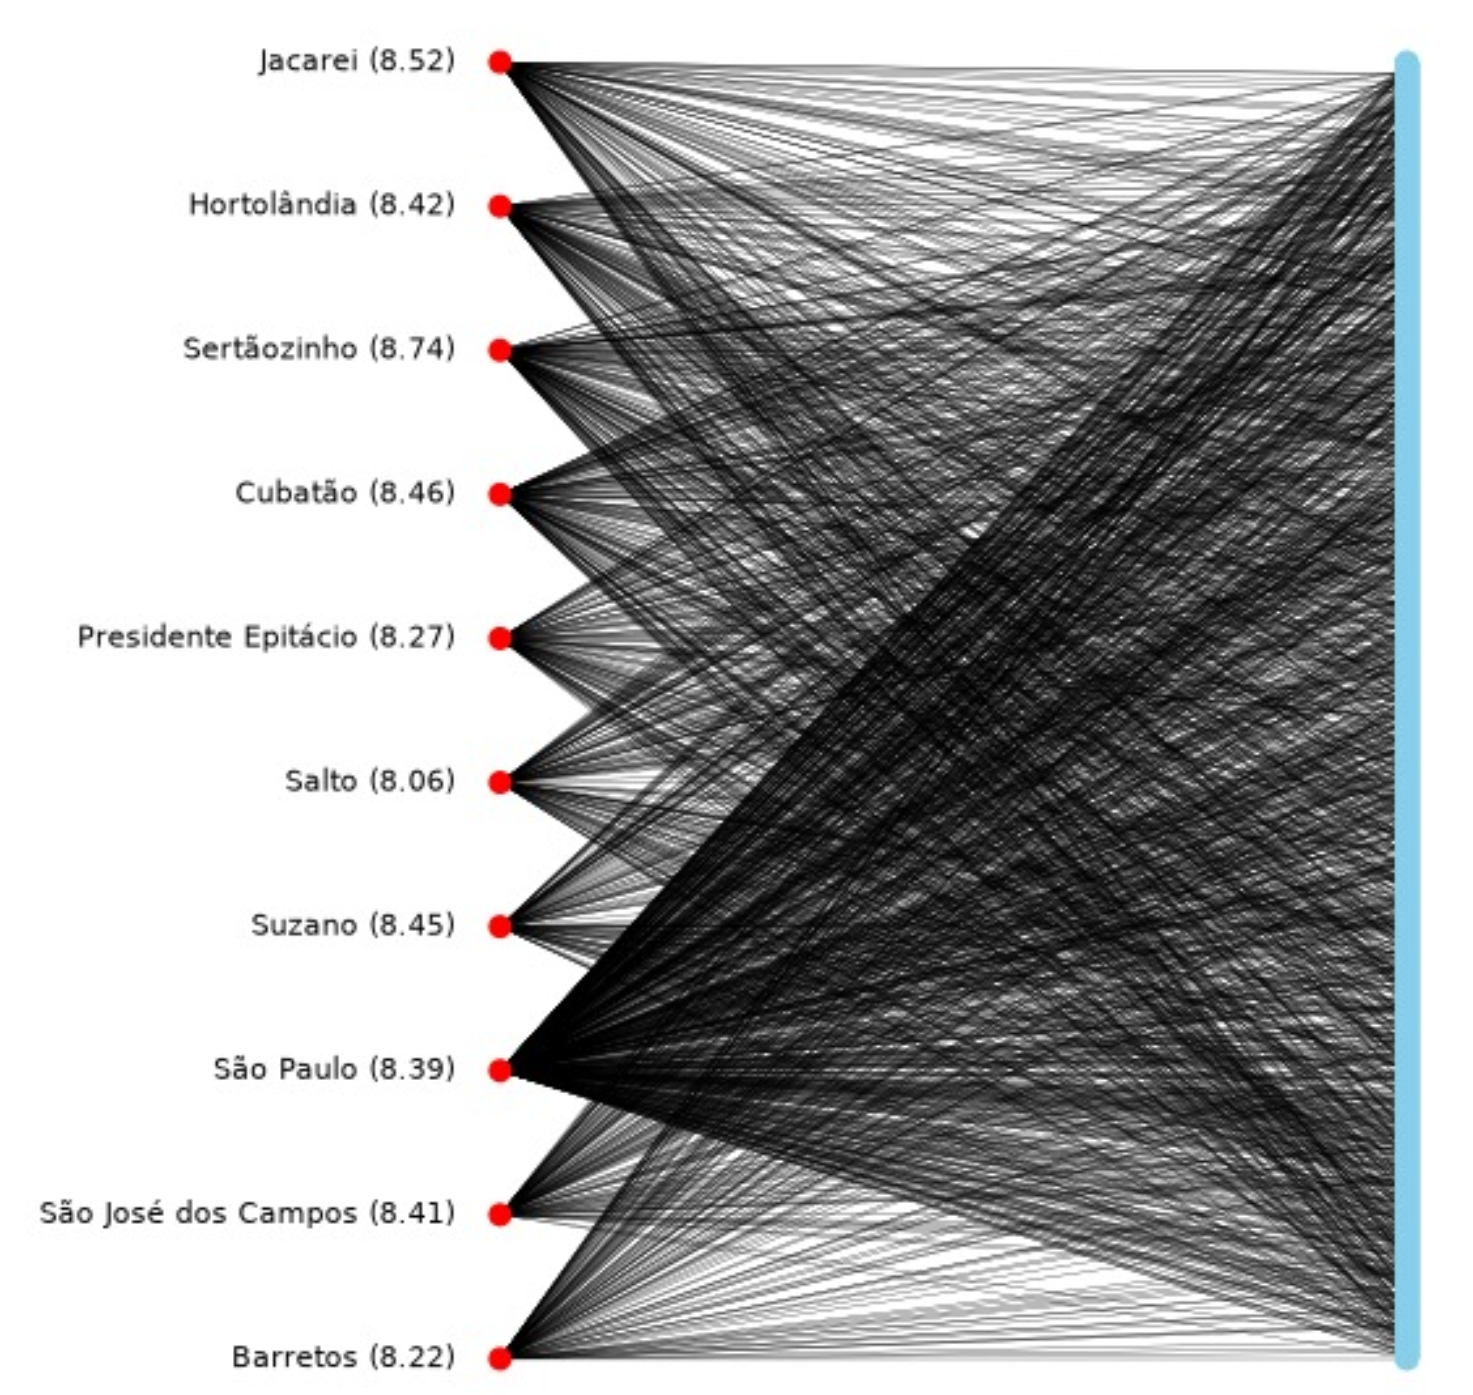
\includegraphics[width=0.7\textwidth]{images/1.png}
    \caption{Grafo dos dados originais}
    \label{fig:grafo}
\end{figure}

\begin{figure}[H]
    \centering
    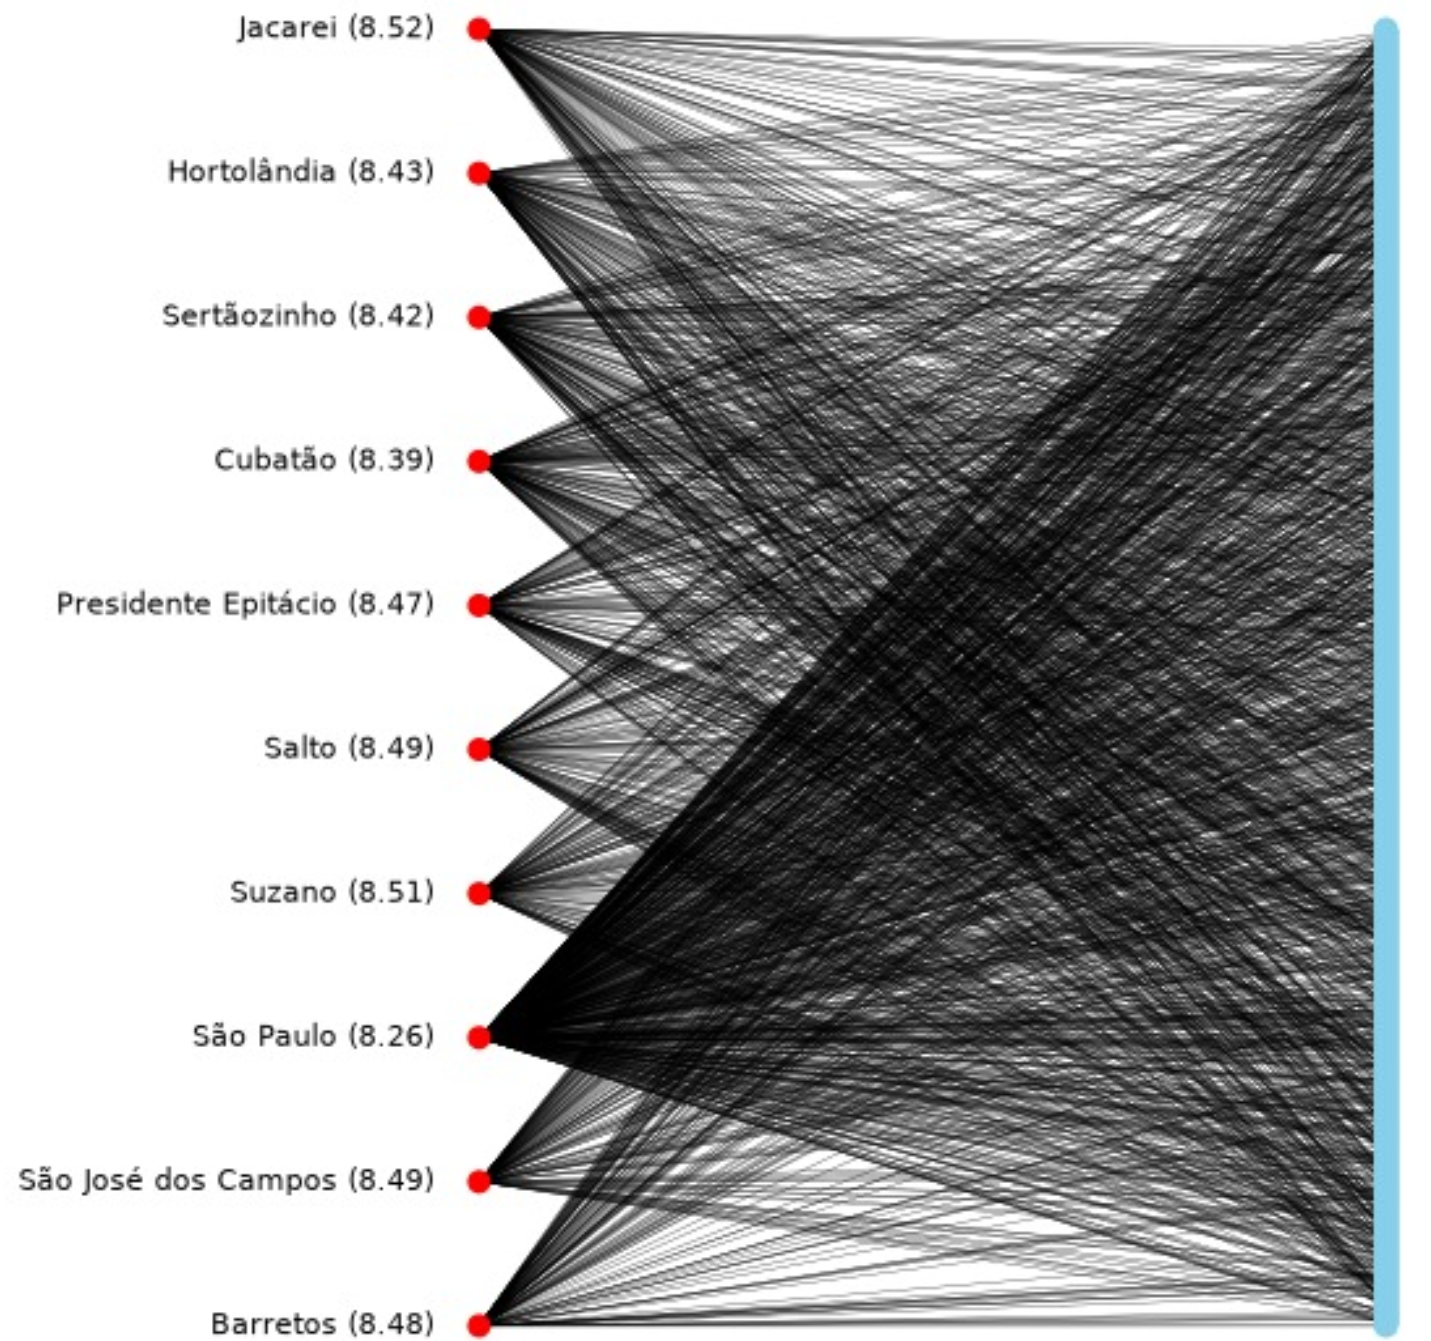
\includegraphics[width=0.7\textwidth]{images/2.png}
    \caption{Alocação do modelo final 1}
    \label{grafo_ex}
\end{figure}


\begin{figure}[H]
    \centering
    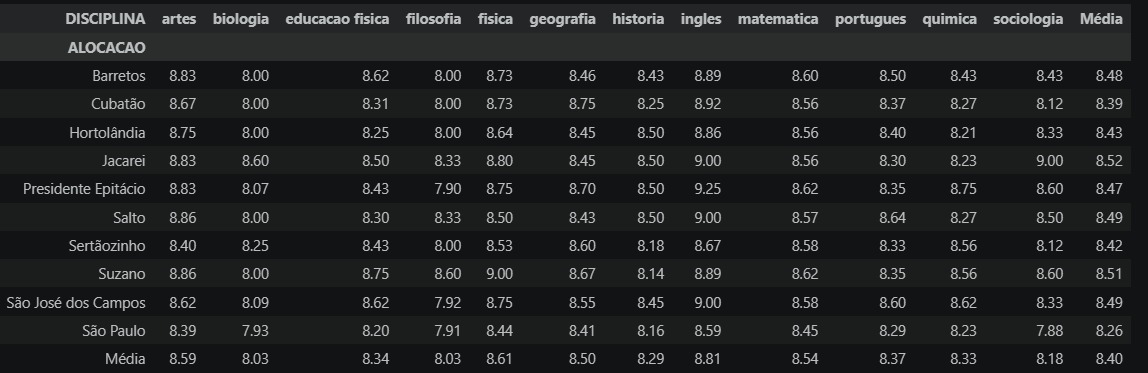
\includegraphics[width=0.7\textwidth]{images/3.png}
    \caption{Tabela de índices de qualidade geral de cada matéria da alocação do modelo final 1 }
    \label{grafo_exemplo}
\end{figure}

\begin{figure}[H]
    \centering
    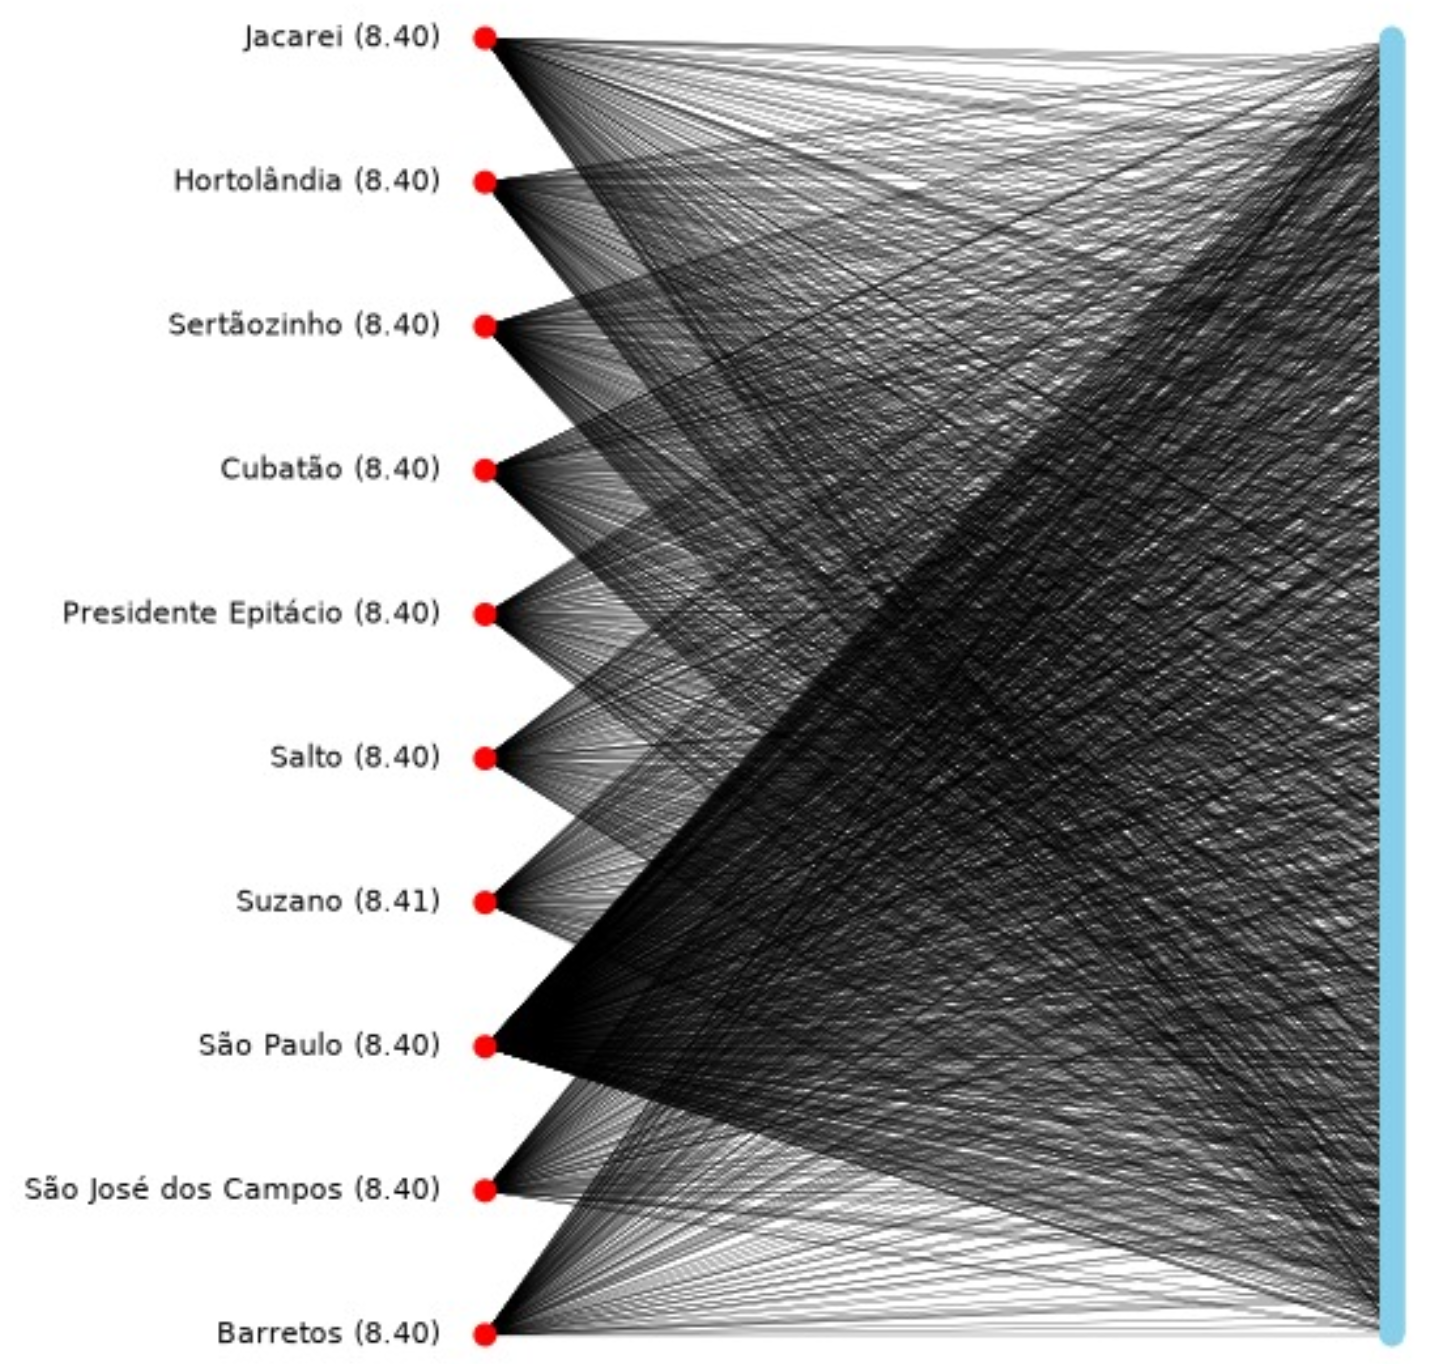
\includegraphics[width=0.7\textwidth]{images/4.png}
    \caption{Alocação do modelo final 2}
    \label{exemplo}
\end{figure}


Dados os números de professores e seus respectivos pesos, obtivemos que o valor $W^*/D$ para esse grafo é $8{,}4$; a segunda alocação obtém um grau mínimo exatamente igual a esse valor, o que significa que o modelo final 2 alcançou seu objetivo com um resultado excelente. O modelo final 1 realiza seu objetivo de forma não tão excelente quanto o segundo, mas ainda alcança um resultado satisfatório, obtendo índices mínimos próximos dos limites superiores da relação da Proposição~\ref{prop:3}.

Esses resultados nos permitem não apenas visualizar o funcionamento do modelo, mas também deixam mais claro em quais situações a lógica da alocação sucessiva para as escolas mais necessitadas funciona melhor. Note que, quando existem muitos professores e muitas vagas para serem alocados e preenchidas, fica mais fácil para o algoritmo balancear esse valor, pois com mais alocações existem mais oportunidades de equilibrar os valores de todas as escolas em torno de um valor médio ($8{,}4$, nesse caso). Isso é exatamente o que acontece com o modelo final 2 e explica seu resultado excelente; já na aplicação do modelo final 1, devido às quantidades bem menores de vagas e professores de uma matéria específica em relação ao todo, seus resultados não são tão precisos quanto os do segundo modelo, justamente por ter menos oportunidades de equilibrar os níveis.

Isso nos dá uma relação muito interessante: algoritmos de enumeração como o \emph{solver} são muito custosos, então são úteis em casos pequenos, mas impraticáveis em números maiores, que é quase a situação contrária da nossa heurística, que funciona muito bem em casos de grandes números, mas é pouco precisa quando existem poucos valores. Portanto, é válido afirmar que os nossos modelos alcançam de forma satisfatória o nosso objetivo de impedir a hiperconcentração de professores de excelência com um método aplicável computacionalmente.


\section{Outras aplicações}

Embora tenha sido desenvolvido para a organização educacional, o modelo não depende de nada específico de professores ou escolas. Ele usa apenas três ingredientes: um conjunto de itens com um valor (os professores, com peso $\delta(p)$), um conjunto de destinos com uma demanda (as escolas, com demandas $q(s,k)$) e o objetivo de elevar o grau do destino em pior situação, isto é, maximizar o menor grau $\delta(s)$. Sempre que um problema tem essa forma, o grafo bipartido $G = (P \cup E, A)$, os algoritmos e as proposições deste trabalho se aplicam sem alterações. Três exemplos ilustram isso.

\paragraph{Saúde.} Considere a distribuição de médicos entre unidades de saúde. Cada médico é um vértice de $P$, com peso $\delta(p)$ calculado a partir de sua formação e experiência, e cada unidade é um vértice de $E$, que demanda $q(s,k)$ médicos de cada especialidade $k$ (por exemplo, pediatria e clínica geral). Maximizar o menor grau evita que uma unidade fique com um quadro muito mais fraco que as demais. A Proposição~\ref{prop:1} indica se há médicos suficientes em cada especialidade para atender a todas as demandas, e a Proposição~\ref{prop:3} fornece o teto $W^*/|E|$ para avaliar a distribuição obtida.

\paragraph{Distribuição de suprimentos.} Em uma emergência, lotes de suprimentos com utilidades diferentes devem ser enviados a abrigos. Cada lote é um vértice de $P$, com $\delta(p)$ representando o seu valor (por exemplo, o número de pessoas que ele atende), e cada abrigo é um vértice de $E$, que comporta $q(s,k)$ lotes de cada tipo $k$ (alimentos, medicamentos, água). Maximizar o menor grau significa priorizar o abrigo mais mal abastecido. É a aplicação em que o critério do modelo, proteger a pior situação, coincide diretamente com o objetivo do problema.

\paragraph{Problemas relacionados.} Se retirarmos as demandas, o modelo vira o problema de distribuir tarefas de durações diferentes entre máquinas idênticas, de modo que a máquina com menos trabalho receba o máximo possível, o que serve para evitar ociosidade. A redução da Partição apresentada neste trabalho se aplica igualmente a esse caso, e por isso os mesmos métodos (a heurística gulosa, a PLI e o limite da Proposição~\ref{prop:3}) valem para ele.


\section{Conclusões conceituais}

\subsection{Grafos bipartidos e emparelhamentos}

Um grafo é bipartido quando seus vértices se dividem em dois grupos sem elementos em comum e toda aresta liga vértices de grupos diferentes. É exatamente o nosso caso: em $G = (P \cup E, A)$, os professores ficam de um lado, as escolas do outro, e uma aresta $\{p, s\}$ representa a alocação do professor $p$ à escola $s$. Nenhuma aresta liga dois professores ou duas escolas, o que reflete o problema real. Com essa estrutura, uma alocação válida $f$ é a escolha de um conjunto de arestas em que cada professor aparece no máximo uma vez e cada escola recebe exatamente a quantidade $q(s,k)$ pedida em cada matéria.

Isso é uma versão do que a teoria chama de emparelhamento, um conjunto de arestas em que nenhum vértice se repete. Para enxergá-lo, basta desdobrar cada escola em vagas, de modo que a escola que pede $2$ professores de Matemática passa a ter duas vagas distintas dessa matéria. Preencher as demandas é então emparelhar cada vaga com um professor diferente.

O teorema de Hall diz quando isso é possível: todas as vagas podem ser preenchidas se, e somente se, para todo grupo $X$ de vagas, o número de professores que podem ocupar pelo menos uma vaga de $X$ (o conjunto $N(X)$, a vizinhança de $X$) for maior ou igual a $|X|$. Na Proposição~\ref{prop:1} essa condição se reduz a uma simples contagem, $|P_k| \ge Q_k$, porque todo professor de uma matéria atende a qualquer vaga dessa mesma matéria, e o grupo mais restritivo é sempre o das vagas de uma única matéria. Se um professor lecionasse duas matérias, ou se houvesse restrições como a distância entre professor e escola, o conjunto $N(X)$ deixaria de ser tão simples e seria preciso verificar a condição de Hall completa. Essa é uma das extensões que apontamos nas limitações do trabalho.

\subsection{Otimização combinatória e complexidade}

A otimização combinatória estuda como escolher a melhor opção entre um conjunto finito de possibilidades. A Proposição~\ref{prop:2} mostra que estamos nessa situação: as alocações válidas são finitas e, por isso, existe uma que maximiza o menor grau ponderado. O problema é que esse conjunto cresce de forma explosiva, pois há até $(|E| + 1)^{|P|}$ funções de $P$ em $E \cup \{\varnothing\}$, e testar todas deixa de ser viável quando o número de professores aumenta.

Isso não é só uma limitação do nosso método. Para ver isso, reduzimos o nosso problema à Partição (Garey e Johnson, 1979). Dados inteiros $a_1, \dots, a_n$ ($n$ par) com soma $S$, é possível separá-los em dois grupos com o mesmo número de elementos e soma $S/2$? Basta tomar duas escolas, cada uma com demanda $n/2$, e $n$ professores com $\delta(p_i) = a_i$. Como todos os professores são alocados, $\delta(s_1) + \delta(s_2) = S$, e então o menor grau não passa de $S/2$, valendo $z = S/2$ se, e somente se, a resposta da Partição é ``sim''. Assim, um algoritmo rápido de tempo polinomial para calcular $z$ resolveria também a Partição, para a qual não se conhece algoritmo desse tipo. Isso significa que o problema é NP-difícil, ou seja, é pelo menos tão difícil quanto os problemas de uma classe famosa, chamada NP, cujas soluções se conferem rapidamente. Essa dificuldade justifica o uso de duas estratégias complementares: a heurística, apresentada no modelo base, que é rápida mas sem garantia de ótimo, e a PLI, apresentada nos modelos finais, que garante o ótimo, mas pode ser exponencial no pior caso.

Dentro do mesmo grafo, o objetivo muda a dificuldade. Maximizar a soma $T(f)$, em vez do menor grau, é um problema de emparelhamento de peso máximo com demandas (um emparelhamento em que a soma dos pesos das arestas é a maior possível), que pode ser resolvido em tempo polinomial por um fluxo de custo mínimo, isto é, escolhendo, entre todas as formas de enviar os professores às vagas, a de menor custo total, com custo igual ao peso do professor com o sinal trocado. Já maximizar o menor grau é NP-difícil, o que mostra que equilibrar as escolas é mais difícil do que apenas maximizar o nível total.


\section{Limitações e possíveis extensões}

\paragraph{O nível dos professores.} Todo o resultado depende do peso $\delta(p)$, que aqui é calculado apenas a partir da formação descrita no currículo. Isso deixa de fora a experiência em sala de aula e a trajetória profissional, e a escala numérica escolhida (por exemplo, doutorado valendo mais que mestrado) é uma decisão nossa, não uma medida objetiva de qualidade. Uma extensão natural é incorporar a carreira ao cálculo do peso e testar o quanto a alocação ótima muda quando a escala muda.

\paragraph{Uma matéria por professor.} Assumimos que cada professor pertence a uma única matéria. É isso que permite que o Modelo Final 1 seja resolvido matéria por matéria, de forma independente, e que a Proposição~\ref{prop:1} se reduza à contagem $|P_k| \ge Q_k$. Se um professor puder lecionar duas matérias, ele ainda só pode estar em uma escola, e as matérias deixam de ser independentes entre si. Nesse caso é preciso verificar a condição de Hall completa, mencionada nas conclusões conceituais, e resolver as matérias em conjunto, o que torna o problema maior.

\paragraph{Fatores humanos e geográficos.} Realocar professores implica deslocamento, vínculo com a instituição e preferências pessoais, e nenhum desses fatores aparece nos modelos. A distância entre a residência do professor e a escola, por exemplo, poderia restringir quais arestas $\{p, s\}$ existem em $G$. Essa é a extensão que mais aproxima o modelo de uma aplicação real, e também a que mais complica o seu uso prático.

\paragraph{O critério de equilíbrio.} Maximizar o menor grau só considera a escola em pior situação e ignora as demais: duas alocações com o mesmo menor grau podem ter escolas muito mais desiguais entre si. Existem métodos alternativos, como minimizar a variância (uma medida do quanto os graus se afastam da média) ou a diferença entre o maior e o menor grau. Existe ainda o critério \emph{leximin}, que maximiza o menor grau, depois o segundo menor, e assim por diante. Todos eles são tão difíceis de resolver quanto o nosso. Além disso, como as escolas têm demandas diferentes, o grau total favorece as que pedem mais professores, e por isso os modelos finais utilizam o índice de qualidade geral $n(s)$, que compara o grau médio por vaga, mantendo as contas lineares.

\paragraph{Os dados.} Utilizamos os institutos federais da região metropolitana de São Paulo e, em parte das simulações, valores estimados. Os resultados mostram o comportamento do modelo, mas não substituem uma validação com dados reais completos e com a participação de quem conhece a gestão dessas instituições.


\section{Conclusão}

Este trabalho propôs um modelo de organização educacional baseado em um grafo bipartido, em que professores e escolas são os vértices e as arestas representam as alocações, com o objetivo de reduzir a hiperconcentração de bons professores em poucas instituições. Para isso, buscamos maximizar o menor grau ponderado das escolas, ou o menor índice de qualidade geral quando as demandas por vagas são muito diferentes.

Mostramos que o objetivo é matematicamente possível: existe alocação válida quando há professores suficientes em cada matéria (Proposição~\ref{prop:1}), existe uma alocação ótima, pois o conjunto de alocações válidas é finito (Proposição~\ref{prop:2}), e o valor ótimo é limitado superiormente por $W^*/|E|$, ou por $W^*/D$ no caso do índice de qualidade (Proposição~\ref{prop:3}), o que permite avaliar a qualidade de qualquer alocação. Também vimos que o problema é NP-difícil, o que justifica o uso conjunto de uma heurística, rápida mas sem garantia de ótimo, e da Programação Linear Inteira, que garante o ótimo.

Os três modelos, o modelo base e os dois modelos finais, mostram como as restrições estruturais, a demanda total por escola e a demanda por matéria, alteram o problema sem mudar o grafo nem o objetivo. Por fim, o mesmo modelo se aplica a outros problemas em que o objetivo é proteger o destino em pior situação, e as limitações apontadas, como o nível dos professores e os fatores humanos e geográficos, indicam caminhos para trabalhos futuros.

\vspace{\baselineskip}

\section*{Referências}

\paragraph{Dados dos institutos federais}

Portal de Dados Abertos do IFSP (conjunto de dados de servidores): \url{https://dados.ifsp.edu.br/id/dataset/servidores}

\paragraph{Grafos bipartidos, emparelhamento e teorema de Hall}
\begin{itemize}
  \item SBMAC, III CMAC-SE, 2015 (artigo sobre emparelhamento em grafos): \url{https://proceedings.sbmac.org.br/sbmac/article/download/941/954/1902}
  \item Mota (UFC, 2009), dissertação ``Uma Generalização do Teorema de Hall e Suas Implicações Para a Teoria de Fatores'': \url{https://mdcc.ufc.br/wp-content/uploads/2024/08/110.-guilherme-oliveira-mota.pdf}
  \item Fernandes (IME-USP), MAC0325, aula 12: \url{https://www.ime.usp.br/~coelho/mac0325-2008/aulas/aula12.pdf}
  \item Netto e Silva (UFG), ``Alocação de salas usando fluxo máximo de custo mínimo em grafos bipartidos'' (SBC): \url{https://sol.sbc.org.br/index.php/erigo/article/download/13867/13714}
  \item UFU, TCC ``O problema de alocação de tarefas e o método húngaro'': \url{https://repositorio.ufu.br/bitstream/123456789/46525/1/problemaAloca%c3%a7%c3%a3oTarefas.pdf}
\end{itemize}

\paragraph{Complexidade e NP-dificuldade (Partição)}
\begin{itemize}
  \item Fernandes (IME-USP), slides de Algoritmos, aula 24: \url{https://www.ime.usp.br/~cris/aulas/13_1_338/slides/aula24.pdf}
  \item Souza (UNICAMP), slides de MO420, aula 07: \url{https://ic.unicamp.br/~ra063658/disciplinas/cic111_2024s1/aula07-handout.pdf}
\end{itemize}

\paragraph{Maximizar o menor valor}
\begin{itemize}
  \item Wikipédia, ``Egalitarian item allocation'': \url{https://en.wikipedia.org/wiki/Egalitarian_item_allocation}
  \item Feige, ``On Allocations that Maximize Fairness'': \url{https://www.wisdom.weizmann.ac.il/~feige/mypapers/santaclaus.pdf}
  \item Bansal e Sviridenko, ``The Santa Claus Problem'' (STOC 2006): \url{https://ics.uci.edu/~theory/269/060609.html}
  \item Walter (2013), CEJOR 21, 125--139: \url{https://core.ac.uk/download/224756799.pdf}
  \item Lawrinenko, Schwerdfeger e Walter (2018), J. Heuristics 24, 173--203: \url{https://link.springer.com/article/10.1007/s10732-017-9362-9}
  \item Bansal e Sviridenko, ``The Santa Claus Problem'' (STOC 2006): \url{https://research.ibm.com/publications/the-santa-claus-problem}
\end{itemize}

\paragraph{PLI (solver)}
\begin{itemize}
  \item Miyazawa (UNICAMP), ``Introdução a Programação Linear e Inteira'': \url{https://ic.unicamp.br/~fkm/lectures/slides-progint.pdf}
  \item Souza (UFOP), notas de aula de Otimização Combinatória: \url{https://www.cos.ufrj.br/~daniel/iECI-2018/slides/Apostila_Otimizacao_Marcone.pdf}
  \item Munari (UFSCar), tópico 7.2: \url{https://dep.ufscar.br/munari/otm2025/slidesTopico7-2.pdf}
  \item Documentação do SciPy, \texttt{scipy.optimize.milp}: \url{https://docs.scipy.org/doc/scipy/reference/generated/scipy.optimize.milp.html}
\end{itemize}

\end{document}